\originalchapter{8.05 作业1：波函数与三个点势}
来源为Fall 2013 Assignment 1, 2013年9月4日发布, 9月13日15时截止. 本篇转述第1--6题, 解答均为\textbf{AI独立解答}. 第2题署Griffiths变题, 第4题参考其方井讨论, 以下按MIT已有模型独立推导并自绘图, 不复制未附的书图. 第7题只有Griffiths 2.38题号, 不补造题面.
\originalsection{第1题：Gaussian乘一次多项式}
\begin{exercise}
$\psi=Nx\e^{-\alpha x^2/2}$,$\alpha>0$. 求归一化及$x,x^2,p,p^2$均值; 判断是否为位置或动量本征态; 自由时求平均能量. 若它是未知势的能量本征态且$V(0)=0$, 求势和能量并判断是否为基态.
\end{exercise}
\begin{solution}
$\int x^2\e^{-\alpha x^2}\dd x=\sqrt\pi/(2\alpha^{3/2})$, 故可取$N=\sqrt2\alpha^{3/4}/\pi^{1/4}$. 密度偶、波函数实使$\langle x\rangle=\langle p\rangle=0$. 连续两次对Gaussian积分参数求导给$\langle x^2\rangle=3/(2\alpha)$, 而$\psi''=(\alpha^2x^2-3\alpha)\psi$, 所以$\langle p^2\rangle=3\hbar^2\alpha/2$. 两方差均非零, 非位置或动量本征态. 自由时$\langle H\rangle=3\hbar^2\alpha/(4m)$, 不能从均值反推能量确定.

对$x\ne0$, 本征方程反解$V=E+\hbar^2(\alpha^2x^2-3\alpha)/(2m)$. 连续势的$V(0)=0$给$E=3\hbar^2\alpha/(2m)$及$V=\hbar^2\alpha^2x^2/(2m)$, 是$\omega=\hbar\alpha/m$谐振子的第一激发态. 原点有一个节点, 因而不是正规一维井的基态. 此处默认普通连续乘法势; 单点改值、奇异势或不同自伴边界条件不能由该反演唯一判定.
\end{solution}
\originalsection{第2题：束缚能量严格高于势的下界}
\begin{exercise}
实势满足$V(x)\ge V_{\min}$, 非零正规束缚本征态可选实. 用微分方程与积分证明$E>V_{\min}$. 原件注明是Griffiths题的变式.
\end{exercise}
\begin{solution}
假设$E\le V_{\min}$, 方程为$\psi''=2m(V-E)\psi/\hbar^2$. 在正规动能形式域中分部积分, 衰减边界项消失, 得
\[
-\int|\psi'|^2\dd x=\frac{2m}{\hbar^2}\int(V-E)|\psi|^2\dd x\ge0.
\]
左侧非正, 所以两侧只能同时为0. $\psi'=0$几乎处处使$\psi$为常数, 全直线上非零常数不能平方可积, 矛盾. 这也说明严格性来自动能不能为0, 不能只以$\langle V\rangle\ge V_{\min}$证明非严格界就结束. 奇异势或别的边界条件必须另检查动能域.
\end{solution}
\originalsection{第3题：三个吸引点势}
\begin{exercise}
$V=-V_0a\sum_{n=-1}^{1}\delta(x-na)$,$V_0,a>0$. 求三点处导数跳跃. 束缚态可否在$x>a$、$0<x<a$或$x=a,0$有节点? 足够强时有几束缚态并给定性形状. 求最低奇态的能量方程和存在阈值.
\end{exercise}
\begin{solution}
设$g=V_0a$, 各点积分方程得$\psi'(na+)-\psi'(na-)=-2mg\psi(na)/\hbar^2$. $E=-\hbar^2\kappa^2/(2m)$时外区只能是衰减指数, 无节点. 无势中段$\psi=A\e^{\kappa x}+B\e^{-\kappa x}$至多一个零点, 因为零点条件$\e^{2\kappa x}=-B/A$只有一个正解. $x=a$不能为节点: 外侧衰减系数将为0, 连续与跳跃条件又给内侧函数和导数都0, 唯一性使整态为0. 原点可以是奇态的节点, 奇态此处点势不发生作用.

最多3个负能态可直接用变分反证: 若有4个独立负能态, 在其四维张成空间能选非零线性组合使三点值都0. 该态点势能0、动能非负, 却在负能本征子空间有严格负的能量均值, 矛盾. 强吸引时选三个不交叠、分别以各中心为峰的试函数, 每个势项随$g$降至负能, 其三维组合全为负, min--max原理给至少3态. 其理由是若负本征态少于试探子空间维数, 可选子空间非零矢正交于全部负态, 其谱能均值非负, 与全负Rayleigh商矛盾. 更具体, 各点值$c_i$满足$c_i=(mg/\hbar^2\kappa)\sum_j\e^{-\kappa|x_i-x_j|}c_j$, 这是三个独立中心的$3\times3$方程. 强吸引时每个中心有一个局域基态, 三个微小耦合组合产生3束缚态. 按节点排序依次为全正偶态、原点一节点奇态、左右各一节点的偶态; 第二偶态中间瓣与两侧瓣异号.

奇态在$0<x<a$写$C\sinh\kappa x$, $x>a$为$D\e^{-\kappa(x-a)}$. 连续和跳跃得$\kappa(1+\coth\kappa a)=2mg/\hbar^2$. 令$s=\kappa a$, $\lambda=mV_0a^2/\hbar^2$, 化为$s=\lambda(1-\e^{-2s})$. 右侧小$s$斜率$2\lambda$, 存在正根恰当$\lambda>1/2$, 即$V_0>\hbar^2/(2ma^2)$. 等号只有不归一阈值态. 对称点值矩阵的奇向量$(1,0,-1)$也给同方程, 可核验导数接续.
\end{solution}
本图取$\lambda=mV_0a^2/\hbar^2=3$, $n=0,1,2$按低到高能量排序.
\begin{center}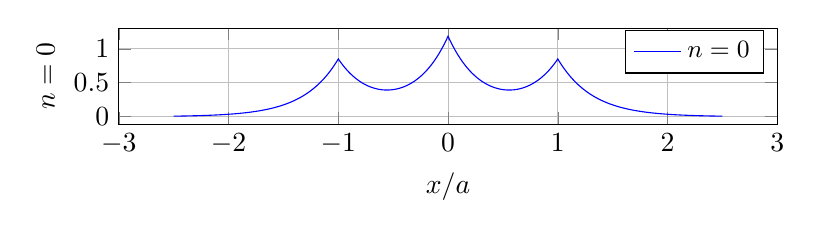
\begin{tikzpicture}
\begin{axis}[width=.82\textwidth,height=2.8cm,xlabel={$x/a$},ylabel={$n=0$},grid=major,legend style={font=\small},]
\addplot+[mark=none] coordinates{(-2.5,0.0072204064) (-2.4875,0.00751312243) (-2.475,0.00781770521) (-2.4625,0.0081346358) (-2.45,0.00846441479) (-2.4375,0.00880756305) (-2.425,0.00916462259) (-2.4125,0.00953615735) (-2.4,0.00992275417) (-2.3875,0.0103250237) (-2.375,0.0107436012) (-2.3625,0.0111791479) (-2.35,0.0116323518) (-2.3375,0.0121039285) (-2.325,0.0125946231) (-2.3125,0.0131052104) (-2.3,0.013636497) (-2.2875,0.014189322) (-2.275,0.0147645587) (-2.2625,0.0153631154) (-2.25,0.0159859377) (-2.2375,0.0166340093) (-2.225,0.0173083538) (-2.2125,0.0180100363) (-2.2,0.0187401651) (-2.1875,0.0194998933) (-2.175,0.0202904211) (-2.1625,0.0211129969) (-2.15,0.02196892) (-2.1375,0.0228595423) (-2.125,0.0237862705) (-2.1125,0.0247505685) (-2.1,0.0257539591) (-2.0875,0.0267980273) (-2.075,0.0278844222) (-2.0625,0.0290148596) (-2.05,0.030191125) (-2.0375,0.0314150764) (-2.025,0.0326886469) (-2.0125,0.0340138481) (-2,0.0353927731) (-1.9875,0.0368275998) (-1.975,0.0383205946) (-1.9625,0.0398741155) (-1.95,0.0414906164) (-1.9375,0.0431726503) (-1.925,0.0449228741) (-1.9125,0.0467440521) (-1.9,0.0486390609) (-1.8875,0.0506108936) (-1.875,0.0526626645) (-1.8625,0.0547976145) (-1.85,0.0570191155) (-1.8375,0.0593306765) (-1.825,0.0617359483) (-1.8125,0.0642387302) (-1.8,0.066842975) (-1.7875,0.0695527963) (-1.775,0.072372474) (-1.7625,0.0753064617) (-1.75,0.0783593935) (-1.7375,0.0815360916) (-1.725,0.0848415733) (-1.7125,0.0882810596) (-1.7,0.0918599831) (-1.6875,0.0955839965) (-1.675,0.0994589817) (-1.6625,0.103491059) (-1.65,0.107686598) (-1.6375,0.112052224) (-1.625,0.116594833) (-1.6125,0.121321599) (-1.6,0.12623999) (-1.5875,0.131357772) (-1.575,0.13668303) (-1.5625,0.142224175) (-1.55,0.147989958) (-1.5375,0.153989486) (-1.525,0.160232236) (-1.5125,0.166728068) (-1.5,0.173487241) (-1.4875,0.180520432) (-1.475,0.187838749) (-1.4625,0.195453752) (-1.45,0.203377468) (-1.4375,0.211622412) (-1.425,0.220201607) (-1.4125,0.229128603) (-1.4,0.2384175) (-1.3875,0.248082971) (-1.375,0.258140281) (-1.3625,0.268605315) (-1.35,0.279494603) (-1.3375,0.290825343) (-1.325,0.302615433) (-1.3125,0.314883495) (-1.3,0.327648905) (-1.2875,0.340931826) (-1.275,0.354753238) (-1.2625,0.369134971) (-1.25,0.384099742) (-1.2375,0.399671186) (-1.225,0.415873898) (-1.2125,0.432733469) (-1.2,0.45027653) (-1.1875,0.468530788) (-1.175,0.487525075) (-1.1625,0.507289393) (-1.15,0.527854958) (-1.1375,0.549254254) (-1.125,0.571521079) (-1.1125,0.594690603) (-1.1,0.618799423) (-1.0875,0.643885617) (-1.075,0.669988807) (-1.0625,0.697150224) (-1.05,0.725412767) (-1.0375,0.754821077) (-1.025,0.785421603) (-1.0125,0.817262678) (-1,0.850394593) (-0.9875,0.821073296) (-0.975,0.793048858) (-0.9625,0.766277016) (-0.95,0.740715484) (-0.9375,0.716323888) (-0.925,0.693063704) (-0.9125,0.670898192) (-0.9,0.649792342) (-0.8875,0.629712819) (-0.875,0.610627907) (-0.8625,0.592507462) (-0.85,0.575322865) (-0.8375,0.559046971) (-0.825,0.543654074) (-0.8125,0.529119862) (-0.8,0.515421378) (-0.7875,0.502536986) (-0.775,0.490446335) (-0.7625,0.479130328) (-0.75,0.468571093) (-0.7375,0.45875195) (-0.725,0.449657392) (-0.7125,0.441273054) (-0.7,0.433585692) (-0.6875,0.426583165) (-0.675,0.420254413) (-0.6625,0.414589439) (-0.65,0.409579296) (-0.6375,0.405216071) (-0.625,0.401492872) (-0.6125,0.398403818) (-0.6,0.39594403) (-0.5875,0.394109623) (-0.575,0.3928977) (-0.5625,0.392306346) (-0.55,0.392334628) (-0.5375,0.39298259) (-0.525,0.394251255) (-0.5125,0.396142628) (-0.5,0.398659695) (-0.4875,0.401806433) (-0.475,0.405587812) (-0.4625,0.410009803) (-0.45,0.415079392) (-0.4375,0.420804586) (-0.425,0.427194427) (-0.4125,0.434259008) (-0.4,0.442009488) (-0.3875,0.450458108) (-0.375,0.459618211) (-0.3625,0.469504268) (-0.35,0.480131891) (-0.3375,0.491517868) (-0.325,0.503680181) (-0.3125,0.516638042) (-0.3,0.530411915) (-0.2875,0.545023558) (-0.275,0.560496048) (-0.2625,0.576853824) (-0.25,0.594122722) (-0.2375,0.612330018) (-0.225,0.63150447) (-0.2125,0.651676363) (-0.2,0.672877559) (-0.1875,0.695141543) (-0.175,0.718503481) (-0.1625,0.743000273) (-0.15,0.76867061) (-0.1375,0.795555038) (-0.125,0.82369602) (-0.1125,0.853138004) (-0.1,0.883927492) (-0.0875,0.916113116) (-0.075,0.949745711) (-0.0625,0.9848784) (-0.05,1.02156667) (-0.0375,1.05986848) (-0.025,1.09984431) (-0.0125,1.14155731) (0,1.18507337) (0.0125,1.14155731) (0.025,1.09984431) (0.0375,1.05986848) (0.05,1.02156667) (0.0625,0.9848784) (0.075,0.949745711) (0.0875,0.916113116) (0.1,0.883927492) (0.1125,0.853138004) (0.125,0.82369602) (0.1375,0.795555038) (0.15,0.76867061) (0.1625,0.743000273) (0.175,0.718503481) (0.1875,0.695141543) (0.2,0.672877559) (0.2125,0.651676363) (0.225,0.63150447) (0.2375,0.612330018) (0.25,0.594122722) (0.2625,0.576853824) (0.275,0.560496048) (0.2875,0.545023558) (0.3,0.530411915) (0.3125,0.516638042) (0.325,0.503680181) (0.3375,0.491517868) (0.35,0.480131891) (0.3625,0.469504268) (0.375,0.459618211) (0.3875,0.450458108) (0.4,0.442009488) (0.4125,0.434259008) (0.425,0.427194427) (0.4375,0.420804586) (0.45,0.415079392) (0.4625,0.410009803) (0.475,0.405587812) (0.4875,0.401806433) (0.5,0.398659695) (0.5125,0.396142628) (0.525,0.394251255) (0.5375,0.39298259) (0.55,0.392334628) (0.5625,0.392306346) (0.575,0.3928977) (0.5875,0.394109623) (0.6,0.39594403) (0.6125,0.398403818) (0.625,0.401492872) (0.6375,0.405216071) (0.65,0.409579296) (0.6625,0.414589439) (0.675,0.420254413) (0.6875,0.426583165) (0.7,0.433585692) (0.7125,0.441273054) (0.725,0.449657392) (0.7375,0.45875195) (0.75,0.468571093) (0.7625,0.479130328) (0.775,0.490446335) (0.7875,0.502536986) (0.8,0.515421378) (0.8125,0.529119862) (0.825,0.543654074) (0.8375,0.559046971) (0.85,0.575322865) (0.8625,0.592507462) (0.875,0.610627907) (0.8875,0.629712819) (0.9,0.649792342) (0.9125,0.670898192) (0.925,0.693063704) (0.9375,0.716323888) (0.95,0.740715484) (0.9625,0.766277016) (0.975,0.793048858) (0.9875,0.821073296) (1,0.850394593) (1.0125,0.817262678) (1.025,0.785421603) (1.0375,0.754821077) (1.05,0.725412767) (1.0625,0.697150224) (1.075,0.669988807) (1.0875,0.643885617) (1.1,0.618799423) (1.1125,0.594690603) (1.125,0.571521079) (1.1375,0.549254254) (1.15,0.527854958) (1.1625,0.507289393) (1.175,0.487525075) (1.1875,0.468530788) (1.2,0.45027653) (1.2125,0.432733469) (1.225,0.415873898) (1.2375,0.399671186) (1.25,0.384099742) (1.2625,0.369134971) (1.275,0.354753238) (1.2875,0.340931826) (1.3,0.327648905) (1.3125,0.314883495) (1.325,0.302615433) (1.3375,0.290825343) (1.35,0.279494603) (1.3625,0.268605315) (1.375,0.258140281) (1.3875,0.248082971) (1.4,0.2384175) (1.4125,0.229128603) (1.425,0.220201607) (1.4375,0.211622412) (1.45,0.203377468) (1.4625,0.195453752) (1.475,0.187838749) (1.4875,0.180520432) (1.5,0.173487241) (1.5125,0.166728068) (1.525,0.160232236) (1.5375,0.153989486) (1.55,0.147989958) (1.5625,0.142224175) (1.575,0.13668303) (1.5875,0.131357772) (1.6,0.12623999) (1.6125,0.121321599) (1.625,0.116594833) (1.6375,0.112052224) (1.65,0.107686598) (1.6625,0.103491059) (1.675,0.0994589817) (1.6875,0.0955839965) (1.7,0.0918599831) (1.7125,0.0882810596) (1.725,0.0848415733) (1.7375,0.0815360916) (1.75,0.0783593935) (1.7625,0.0753064617) (1.775,0.072372474) (1.7875,0.0695527963) (1.8,0.066842975) (1.8125,0.0642387302) (1.825,0.0617359483) (1.8375,0.0593306765) (1.85,0.0570191155) (1.8625,0.0547976145) (1.875,0.0526626645) (1.8875,0.0506108936) (1.9,0.0486390609) (1.9125,0.0467440521) (1.925,0.0449228741) (1.9375,0.0431726503) (1.95,0.0414906164) (1.9625,0.0398741155) (1.975,0.0383205946) (1.9875,0.0368275998) (2,0.0353927731) (2.0125,0.0340138481) (2.025,0.0326886469) (2.0375,0.0314150764) (2.05,0.030191125) (2.0625,0.0290148596) (2.075,0.0278844222) (2.0875,0.0267980273) (2.1,0.0257539591) (2.1125,0.0247505685) (2.125,0.0237862705) (2.1375,0.0228595423) (2.15,0.02196892) (2.1625,0.0211129969) (2.175,0.0202904211) (2.1875,0.0194998933) (2.2,0.0187401651) (2.2125,0.0180100363) (2.225,0.0173083538) (2.2375,0.0166340093) (2.25,0.0159859377) (2.2625,0.0153631154) (2.275,0.0147645587) (2.2875,0.014189322) (2.3,0.013636497) (2.3125,0.0131052104) (2.325,0.0125946231) (2.3375,0.0121039285) (2.35,0.0116323518) (2.3625,0.0111791479) (2.375,0.0107436012) (2.3875,0.0103250237) (2.4,0.00992275417) (2.4125,0.00953615735) (2.425,0.00916462259) (2.4375,0.00880756305) (2.45,0.00846441479) (2.4625,0.0081346358) (2.475,0.00781770521) (2.4875,0.00751312243) (2.5,0.0072204064)};
\addlegendentry{$n=0$}
\end{axis}\end{tikzpicture}\end{center}
\begin{center}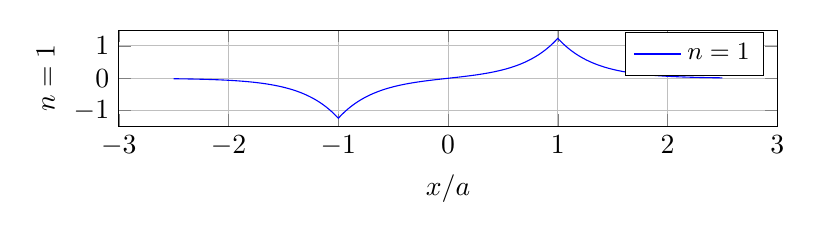
\begin{tikzpicture}
\begin{axis}[width=.82\textwidth,height=2.8cm,xlabel={$x/a$},ylabel={$n=1$},grid=major,legend style={font=\small},]
\addplot+[mark=none] coordinates{(-2.5,-0.0138308173) (-2.4875,-0.0143579655) (-2.475,-0.0149052054) (-2.4625,-0.0154733028) (-2.45,-0.0160630527) (-2.4375,-0.0166752803) (-2.425,-0.0173108424) (-2.4125,-0.0179706284) (-2.4,-0.0186555614) (-2.3875,-0.0193666) (-2.375,-0.0201047392) (-2.3625,-0.0208710118) (-2.35,-0.0216664901) (-2.3375,-0.0224922873) (-2.325,-0.023349559) (-2.3125,-0.0242395047) (-2.3,-0.0251633699) (-2.2875,-0.0261224473) (-2.275,-0.027118079) (-2.2625,-0.0281516582) (-2.25,-0.0292246313) (-2.2375,-0.0303384998) (-2.225,-0.0314948222) (-2.2125,-0.0326952168) (-2.2,-0.0339413632) (-2.1875,-0.0352350053) (-2.175,-0.0365779533) (-2.1625,-0.0379720864) (-2.15,-0.0394193556) (-2.1375,-0.040921786) (-2.125,-0.0424814801) (-2.1125,-0.0441006205) (-2.1,-0.0457814728) (-2.0875,-0.0475263891) (-2.075,-0.0493378113) (-2.0625,-0.051218274) (-2.05,-0.0531704088) (-2.0375,-0.0551969472) (-2.025,-0.0573007253) (-2.0125,-0.0594846867) (-2,-0.0617518878) (-1.9875,-0.064105501) (-1.975,-0.0665488199) (-1.9625,-0.0690852635) (-1.95,-0.0717183812) (-1.9375,-0.0744518576) (-1.925,-0.0772895178) (-1.9125,-0.0802353327) (-1.9,-0.0832934244) (-1.8875,-0.0864680724) (-1.875,-0.0897637189) (-1.8625,-0.0931849759) (-1.85,-0.0967366307) (-1.8375,-0.100423653) (-1.825,-0.104251203) (-1.8125,-0.108224637) (-1.8,-0.112349514) (-1.7875,-0.116631606) (-1.775,-0.121076906) (-1.7625,-0.125691635) (-1.75,-0.13048225) (-1.7375,-0.135455454) (-1.725,-0.140618207) (-1.7125,-0.145977733) (-1.7,-0.151541533) (-1.6875,-0.157317391) (-1.675,-0.16331339) (-1.6625,-0.169537922) (-1.65,-0.175999695) (-1.6375,-0.182707752) (-1.625,-0.189671481) (-1.6125,-0.196900625) (-1.6,-0.204405301) (-1.5875,-0.21219601) (-1.575,-0.220283655) (-1.5625,-0.228679553) (-1.55,-0.237395451) (-1.5375,-0.246443548) (-1.525,-0.255836505) (-1.5125,-0.265587465) (-1.5,-0.275710073) (-1.4875,-0.286218494) (-1.475,-0.297127434) (-1.4625,-0.308452158) (-1.45,-0.320208512) (-1.4375,-0.332412948) (-1.425,-0.345082545) (-1.4125,-0.358235031) (-1.4,-0.371888811) (-1.3875,-0.386062992) (-1.375,-0.400777407) (-1.3625,-0.416052649) (-1.35,-0.431910091) (-1.3375,-0.448371925) (-1.325,-0.465461185) (-1.3125,-0.483201786) (-1.3,-0.501618553) (-1.2875,-0.520737256) (-1.275,-0.540584651) (-1.2625,-0.56118851) (-1.25,-0.582577664) (-1.2375,-0.604782046) (-1.225,-0.627832726) (-1.2125,-0.651761961) (-1.2,-0.676603234) (-1.1875,-0.702391309) (-1.175,-0.729162272) (-1.1625,-0.756953583) (-1.15,-0.785804134) (-1.1375,-0.815754295) (-1.125,-0.846845977) (-1.1125,-0.879122689) (-1.1,-0.912629596) (-1.0875,-0.947413586) (-1.075,-0.983523334) (-1.0625,-1.02100937) (-1.05,-1.05992415) (-1.0375,-1.10032213) (-1.025,-1.14225984) (-1.0125,-1.18579596) (-1,-1.23099142) (-0.9875,-1.18556358) (-0.975,-1.14179474) (-0.9625,-1.09962367) (-0.95,-1.05899136) (-0.9375,-1.01984093) (-0.925,-0.982117618) (-0.9125,-0.945768624) (-0.9,-0.910743086) (-0.8875,-0.876991991) (-0.875,-0.84446811) (-0.8625,-0.813125931) (-0.85,-0.782921596) (-0.8375,-0.753812837) (-0.825,-0.725758923) (-0.8125,-0.698720595) (-0.8,-0.672660017) (-0.7875,-0.647540723) (-0.775,-0.623327562) (-0.7625,-0.59998665) (-0.75,-0.577485327) (-0.7375,-0.555792104) (-0.725,-0.534876626) (-0.7125,-0.514709625) (-0.7,-0.49526288) (-0.6875,-0.476509178) (-0.675,-0.458422277) (-0.6625,-0.440976866) (-0.65,-0.424148534) (-0.6375,-0.407913732) (-0.625,-0.392249742) (-0.6125,-0.377134644) (-0.6,-0.362547288) (-0.5875,-0.34846726) (-0.575,-0.334874858) (-0.5625,-0.321751061) (-0.55,-0.309077505) (-0.5375,-0.296836454) (-0.525,-0.28501078) (-0.5125,-0.273583935) (-0.5,-0.262539927) (-0.4875,-0.251863304) (-0.475,-0.241539124) (-0.4625,-0.23155294) (-0.45,-0.221890779) (-0.4375,-0.212539119) (-0.425,-0.203484875) (-0.4125,-0.194715376) (-0.4,-0.186218351) (-0.3875,-0.17798191) (-0.375,-0.169994526) (-0.3625,-0.162245024) (-0.35,-0.154722558) (-0.3375,-0.147416603) (-0.325,-0.140316934) (-0.3125,-0.133413617) (-0.3,-0.126696991) (-0.2875,-0.120157658) (-0.275,-0.113786467) (-0.2625,-0.107574503) (-0.25,-0.101513072) (-0.2375,-0.0955936933) (-0.225,-0.0898080829) (-0.2125,-0.084148145) (-0.2,-0.0786059593) (-0.1875,-0.0731737704) (-0.175,-0.0678439769) (-0.1625,-0.0626091205) (-0.15,-0.0574618757) (-0.1375,-0.05239504) (-0.125,-0.0474015229) (-0.1125,-0.042474337) (-0.1,-0.0376065872) (-0.0875,-0.032791462) (-0.075,-0.0280222234) (-0.0625,-0.0232921975) (-0.05,-0.0185947654) (-0.0375,-0.0139233538) (-0.025,-0.00927142579) (-0.0125,-0.00463247168) (0,9.58752997e-17) (0.0125,0.00463247168) (0.025,0.00927142579) (0.0375,0.0139233538) (0.05,0.0185947654) (0.0625,0.0232921975) (0.075,0.0280222234) (0.0875,0.032791462) (0.1,0.0376065872) (0.1125,0.042474337) (0.125,0.0474015229) (0.1375,0.05239504) (0.15,0.0574618757) (0.1625,0.0626091205) (0.175,0.0678439769) (0.1875,0.0731737704) (0.2,0.0786059593) (0.2125,0.084148145) (0.225,0.0898080829) (0.2375,0.0955936933) (0.25,0.101513072) (0.2625,0.107574503) (0.275,0.113786467) (0.2875,0.120157658) (0.3,0.126696991) (0.3125,0.133413617) (0.325,0.140316934) (0.3375,0.147416603) (0.35,0.154722558) (0.3625,0.162245024) (0.375,0.169994526) (0.3875,0.17798191) (0.4,0.186218351) (0.4125,0.194715376) (0.425,0.203484875) (0.4375,0.212539119) (0.45,0.221890779) (0.4625,0.23155294) (0.475,0.241539124) (0.4875,0.251863304) (0.5,0.262539927) (0.5125,0.273583935) (0.525,0.28501078) (0.5375,0.296836454) (0.55,0.309077505) (0.5625,0.321751061) (0.575,0.334874858) (0.5875,0.34846726) (0.6,0.362547288) (0.6125,0.377134644) (0.625,0.392249742) (0.6375,0.407913732) (0.65,0.424148534) (0.6625,0.440976866) (0.675,0.458422277) (0.6875,0.476509178) (0.7,0.49526288) (0.7125,0.514709625) (0.725,0.534876626) (0.7375,0.555792104) (0.75,0.577485327) (0.7625,0.59998665) (0.775,0.623327562) (0.7875,0.647540723) (0.8,0.672660017) (0.8125,0.698720595) (0.825,0.725758923) (0.8375,0.753812837) (0.85,0.782921596) (0.8625,0.813125931) (0.875,0.84446811) (0.8875,0.876991991) (0.9,0.910743086) (0.9125,0.945768624) (0.925,0.982117618) (0.9375,1.01984093) (0.95,1.05899136) (0.9625,1.09962367) (0.975,1.14179474) (0.9875,1.18556358) (1,1.23099142) (1.0125,1.18579596) (1.025,1.14225984) (1.0375,1.10032213) (1.05,1.05992415) (1.0625,1.02100937) (1.075,0.983523334) (1.0875,0.947413586) (1.1,0.912629596) (1.1125,0.879122689) (1.125,0.846845977) (1.1375,0.815754295) (1.15,0.785804134) (1.1625,0.756953583) (1.175,0.729162272) (1.1875,0.702391309) (1.2,0.676603234) (1.2125,0.651761961) (1.225,0.627832726) (1.2375,0.604782046) (1.25,0.582577664) (1.2625,0.56118851) (1.275,0.540584651) (1.2875,0.520737256) (1.3,0.501618553) (1.3125,0.483201786) (1.325,0.465461185) (1.3375,0.448371925) (1.35,0.431910091) (1.3625,0.416052649) (1.375,0.400777407) (1.3875,0.386062992) (1.4,0.371888811) (1.4125,0.358235031) (1.425,0.345082545) (1.4375,0.332412948) (1.45,0.320208512) (1.4625,0.308452158) (1.475,0.297127434) (1.4875,0.286218494) (1.5,0.275710073) (1.5125,0.265587465) (1.525,0.255836505) (1.5375,0.246443548) (1.55,0.237395451) (1.5625,0.228679553) (1.575,0.220283655) (1.5875,0.21219601) (1.6,0.204405301) (1.6125,0.196900625) (1.625,0.189671481) (1.6375,0.182707752) (1.65,0.175999695) (1.6625,0.169537922) (1.675,0.16331339) (1.6875,0.157317391) (1.7,0.151541533) (1.7125,0.145977733) (1.725,0.140618207) (1.7375,0.135455454) (1.75,0.13048225) (1.7625,0.125691635) (1.775,0.121076906) (1.7875,0.116631606) (1.8,0.112349514) (1.8125,0.108224637) (1.825,0.104251203) (1.8375,0.100423653) (1.85,0.0967366307) (1.8625,0.0931849759) (1.875,0.0897637189) (1.8875,0.0864680724) (1.9,0.0832934244) (1.9125,0.0802353327) (1.925,0.0772895178) (1.9375,0.0744518576) (1.95,0.0717183812) (1.9625,0.0690852635) (1.975,0.0665488199) (1.9875,0.064105501) (2,0.0617518878) (2.0125,0.0594846867) (2.025,0.0573007253) (2.0375,0.0551969472) (2.05,0.0531704088) (2.0625,0.051218274) (2.075,0.0493378113) (2.0875,0.0475263891) (2.1,0.0457814728) (2.1125,0.0441006205) (2.125,0.0424814801) (2.1375,0.040921786) (2.15,0.0394193556) (2.1625,0.0379720864) (2.175,0.0365779533) (2.1875,0.0352350053) (2.2,0.0339413632) (2.2125,0.0326952168) (2.225,0.0314948222) (2.2375,0.0303384998) (2.25,0.0292246313) (2.2625,0.0281516582) (2.275,0.027118079) (2.2875,0.0261224473) (2.3,0.0251633699) (2.3125,0.0242395047) (2.325,0.023349559) (2.3375,0.0224922873) (2.35,0.0216664901) (2.3625,0.0208710118) (2.375,0.0201047392) (2.3875,0.0193666) (2.4,0.0186555614) (2.4125,0.0179706284) (2.425,0.0173108424) (2.4375,0.0166752803) (2.45,0.0160630527) (2.4625,0.0154733028) (2.475,0.0149052054) (2.4875,0.0143579655) (2.5,0.0138308173)};
\addlegendentry{$n=1$}
\end{axis}\end{tikzpicture}\end{center}
\begin{center}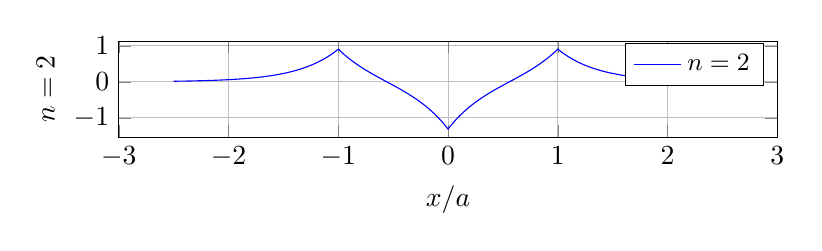
\begin{tikzpicture}
\begin{axis}[width=.82\textwidth,height=2.8cm,xlabel={$x/a$},ylabel={$n=2$},grid=major,legend style={font=\small},]
\addplot+[mark=none] coordinates{(-2.5,0.0151349957) (-2.4875,0.0156602858) (-2.475,0.0162038072) (-2.4625,0.0167661926) (-2.45,0.0173480967) (-2.4375,0.0179501969) (-2.425,0.0185731942) (-2.4125,0.0192178139) (-2.4,0.0198848064) (-2.3875,0.0205749482) (-2.375,0.0212890427) (-2.3625,0.0220279213) (-2.35,0.0227924441) (-2.3375,0.0235835013) (-2.325,0.0244020136) (-2.3125,0.0252489341) (-2.3,0.0261252486) (-2.2875,0.0270319773) (-2.275,0.0279701759) (-2.2625,0.0289409365) (-2.25,0.0299453893) (-2.2375,0.0309847036) (-2.225,0.0320600895) (-2.2125,0.0331727987) (-2.2,0.0343241267) (-2.1875,0.0355154138) (-2.175,0.0367480469) (-2.1625,0.038023461) (-2.15,0.0393431409) (-2.1375,0.0407086229) (-2.125,0.0421214967) (-2.1125,0.0435834071) (-2.1,0.045096056) (-2.0875,0.0466612044) (-2.075,0.0482806743) (-2.0625,0.0499563512) (-2.05,0.0516901858) (-2.0375,0.0534841966) (-2.025,0.0553404721) (-2.0125,0.0572611733) (-2,0.0592485363) (-1.9875,0.0613048747) (-1.975,0.0634325823) (-1.9625,0.0656341364) (-1.95,0.0679120997) (-1.9375,0.0702691243) (-1.925,0.0727079541) (-1.9125,0.0752314284) (-1.9,0.0778424848) (-1.8875,0.0805441632) (-1.875,0.0833396087) (-1.8625,0.0862320756) (-1.85,0.0892249315) (-1.8375,0.0923216603) (-1.825,0.0955258672) (-1.8125,0.0988412826) (-1.8,0.102271766) (-1.7875,0.105821311) (-1.775,0.10949405) (-1.7625,0.113294259) (-1.75,0.117226362) (-1.7375,0.121294936) (-1.725,0.125504719) (-1.7125,0.12986061) (-1.7,0.13436768) (-1.6875,0.139031178) (-1.675,0.143856532) (-1.6625,0.148849359) (-1.65,0.154015473) (-1.6375,0.159360886) (-1.625,0.164891823) (-1.6125,0.170614722) (-1.6,0.176536245) (-1.5875,0.182663287) (-1.575,0.18900298) (-1.5625,0.195562704) (-1.55,0.202350097) (-1.5375,0.20937306) (-1.525,0.216639769) (-1.5125,0.224158683) (-1.5,0.231938556) (-1.4875,0.239988446) (-1.475,0.248317722) (-1.4625,0.256936083) (-1.45,0.265853561) (-1.4375,0.275080538) (-1.425,0.284627756) (-1.4125,0.294506329) (-1.4,0.304727757) (-1.3875,0.31530394) (-1.375,0.326247191) (-1.3625,0.337570249) (-1.35,0.349286296) (-1.3375,0.361408972) (-1.325,0.37395239) (-1.3125,0.386931152) (-1.3,0.400360368) (-1.2875,0.414255671) (-1.275,0.428633239) (-1.2625,0.443509808) (-1.25,0.458902699) (-1.2375,0.474829831) (-1.225,0.491309745) (-1.2125,0.508361627) (-1.2,0.52600533) (-1.1875,0.544261391) (-1.175,0.563151066) (-1.1625,0.582696345) (-1.15,0.602919981) (-1.1375,0.623845519) (-1.125,0.645497319) (-1.1125,0.667900589) (-1.1,0.691081408) (-1.0875,0.715066764) (-1.075,0.739884579) (-1.0625,0.765563746) (-1.05,0.792134159) (-1.0375,0.819626752) (-1.025,0.848073529) (-1.0125,0.877507609) (-1,0.907963257) (-0.9875,0.871365473) (-0.975,0.835782106) (-0.9625,0.801171732) (-0.95,0.767494058) (-0.9375,0.734709878) (-0.925,0.702781026) (-0.9125,0.67167033) (-0.9,0.641341573) (-0.8875,0.611759447) (-0.875,0.582889513) (-0.8625,0.554698161) (-0.85,0.527152573) (-0.8375,0.50022068) (-0.825,0.47387113) (-0.8125,0.448073246) (-0.8,0.422796995) (-0.7875,0.398012953) (-0.775,0.373692265) (-0.7625,0.349806618) (-0.75,0.326328207) (-0.7375,0.303229696) (-0.725,0.280484197) (-0.7125,0.258065229) (-0.7,0.235946693) (-0.6875,0.214102839) (-0.675,0.192508237) (-0.6625,0.171137748) (-0.65,0.149966492) (-0.6375,0.128969823) (-0.625,0.108123297) (-0.6125,0.087402644) (-0.6,0.066783743) (-0.5875,0.0462425897) (-0.575,0.0257552707) (-0.5625,0.00529793512) (-0.55,-0.0151532327) (-0.5375,-0.0356220415) (-0.525,-0.0561323204) (-0.5125,-0.0767079469) (-0.5,-0.0973728745) (-0.4875,-0.118151161) (-0.475,-0.139066995) (-0.4625,-0.160144727) (-0.45,-0.181408895) (-0.4375,-0.202884253) (-0.425,-0.224595804) (-0.4125,-0.246568822) (-0.4,-0.268828888) (-0.3875,-0.291401917) (-0.375,-0.314314187) (-0.3625,-0.337592373) (-0.35,-0.361263573) (-0.3375,-0.385355346) (-0.325,-0.409895738) (-0.3125,-0.434913319) (-0.3,-0.460437213) (-0.2875,-0.486497134) (-0.275,-0.513123421) (-0.2625,-0.540347071) (-0.25,-0.568199776) (-0.2375,-0.596713963) (-0.225,-0.625922827) (-0.2125,-0.655860372) (-0.2,-0.68656145) (-0.1875,-0.718061802) (-0.175,-0.7503981) (-0.1625,-0.78360799) (-0.15,-0.817730133) (-0.1375,-0.852804253) (-0.125,-0.888871182) (-0.1125,-0.925972909) (-0.1,-0.964152626) (-0.0875,-1.00345478) (-0.075,-1.04392513) (-0.0625,-1.08561078) (-0.05,-1.12856027) (-0.0375,-1.1728236) (-0.025,-1.21845229) (-0.0125,-1.26549947) (0,-1.3140199) (0.0125,-1.26549947) (0.025,-1.21845229) (0.0375,-1.1728236) (0.05,-1.12856027) (0.0625,-1.08561078) (0.075,-1.04392513) (0.0875,-1.00345478) (0.1,-0.964152626) (0.1125,-0.925972909) (0.125,-0.888871182) (0.1375,-0.852804253) (0.15,-0.817730133) (0.1625,-0.78360799) (0.175,-0.7503981) (0.1875,-0.718061802) (0.2,-0.68656145) (0.2125,-0.655860372) (0.225,-0.625922827) (0.2375,-0.596713963) (0.25,-0.568199776) (0.2625,-0.540347071) (0.275,-0.513123421) (0.2875,-0.486497134) (0.3,-0.460437213) (0.3125,-0.434913319) (0.325,-0.409895738) (0.3375,-0.385355346) (0.35,-0.361263573) (0.3625,-0.337592373) (0.375,-0.314314187) (0.3875,-0.291401917) (0.4,-0.268828888) (0.4125,-0.246568822) (0.425,-0.224595804) (0.4375,-0.202884253) (0.45,-0.181408895) (0.4625,-0.160144727) (0.475,-0.139066995) (0.4875,-0.118151161) (0.5,-0.0973728745) (0.5125,-0.0767079469) (0.525,-0.0561323204) (0.5375,-0.0356220415) (0.55,-0.0151532327) (0.5625,0.00529793512) (0.575,0.0257552707) (0.5875,0.0462425897) (0.6,0.066783743) (0.6125,0.087402644) (0.625,0.108123297) (0.6375,0.128969823) (0.65,0.149966492) (0.6625,0.171137748) (0.675,0.192508237) (0.6875,0.214102839) (0.7,0.235946693) (0.7125,0.258065229) (0.725,0.280484197) (0.7375,0.303229696) (0.75,0.326328207) (0.7625,0.349806618) (0.775,0.373692265) (0.7875,0.398012953) (0.8,0.422796995) (0.8125,0.448073246) (0.825,0.47387113) (0.8375,0.50022068) (0.85,0.527152573) (0.8625,0.554698161) (0.875,0.582889513) (0.8875,0.611759447) (0.9,0.641341573) (0.9125,0.67167033) (0.925,0.702781026) (0.9375,0.734709878) (0.95,0.767494058) (0.9625,0.801171732) (0.975,0.835782106) (0.9875,0.871365473) (1,0.907963257) (1.0125,0.877507609) (1.025,0.848073529) (1.0375,0.819626752) (1.05,0.792134159) (1.0625,0.765563746) (1.075,0.739884579) (1.0875,0.715066764) (1.1,0.691081408) (1.1125,0.667900589) (1.125,0.645497319) (1.1375,0.623845519) (1.15,0.602919981) (1.1625,0.582696345) (1.175,0.563151066) (1.1875,0.544261391) (1.2,0.52600533) (1.2125,0.508361627) (1.225,0.491309745) (1.2375,0.474829831) (1.25,0.458902699) (1.2625,0.443509808) (1.275,0.428633239) (1.2875,0.414255671) (1.3,0.400360368) (1.3125,0.386931152) (1.325,0.37395239) (1.3375,0.361408972) (1.35,0.349286296) (1.3625,0.337570249) (1.375,0.326247191) (1.3875,0.31530394) (1.4,0.304727757) (1.4125,0.294506329) (1.425,0.284627756) (1.4375,0.275080538) (1.45,0.265853561) (1.4625,0.256936083) (1.475,0.248317722) (1.4875,0.239988446) (1.5,0.231938556) (1.5125,0.224158683) (1.525,0.216639769) (1.5375,0.20937306) (1.55,0.202350097) (1.5625,0.195562704) (1.575,0.18900298) (1.5875,0.182663287) (1.6,0.176536245) (1.6125,0.170614722) (1.625,0.164891823) (1.6375,0.159360886) (1.65,0.154015473) (1.6625,0.148849359) (1.675,0.143856532) (1.6875,0.139031178) (1.7,0.13436768) (1.7125,0.12986061) (1.725,0.125504719) (1.7375,0.121294936) (1.75,0.117226362) (1.7625,0.113294259) (1.775,0.10949405) (1.7875,0.105821311) (1.8,0.102271766) (1.8125,0.0988412826) (1.825,0.0955258672) (1.8375,0.0923216603) (1.85,0.0892249315) (1.8625,0.0862320756) (1.875,0.0833396087) (1.8875,0.0805441632) (1.9,0.0778424848) (1.9125,0.0752314284) (1.925,0.0727079541) (1.9375,0.0702691243) (1.95,0.0679120997) (1.9625,0.0656341364) (1.975,0.0634325823) (1.9875,0.0613048747) (2,0.0592485363) (2.0125,0.0572611733) (2.025,0.0553404721) (2.0375,0.0534841966) (2.05,0.0516901858) (2.0625,0.0499563512) (2.075,0.0482806743) (2.0875,0.0466612044) (2.1,0.045096056) (2.1125,0.0435834071) (2.125,0.0421214967) (2.1375,0.0407086229) (2.15,0.0393431409) (2.1625,0.038023461) (2.175,0.0367480469) (2.1875,0.0355154138) (2.2,0.0343241267) (2.2125,0.0331727987) (2.225,0.0320600895) (2.2375,0.0309847036) (2.25,0.0299453893) (2.2625,0.0289409365) (2.275,0.0279701759) (2.2875,0.0270319773) (2.3,0.0261252486) (2.3125,0.0252489341) (2.325,0.0244020136) (2.3375,0.0235835013) (2.35,0.0227924441) (2.3625,0.0220279213) (2.375,0.0212890427) (2.3875,0.0205749482) (2.4,0.0198848064) (2.4125,0.0192178139) (2.425,0.0185731942) (2.4375,0.0179501969) (2.45,0.0173480967) (2.4625,0.0167661926) (2.475,0.0162038072) (2.4875,0.0156602858) (2.5,0.0151349957)};
\addlegendentry{$n=2$}
\end{axis}\end{tikzpicture}\end{center}

\originalsection{第4题：深方井计数与浅方井能量}
\begin{exercise}
$V=-V_0$于$|x|\le a$, 外为0, 定义$z_0=a\sqrt{2mV_0}/\hbar$. (a)用节点数估计深井束缚态数. (b)求$z_0\ll1$时最低能量首项. 原题参考Griffiths方井图, 此处使用本册自己的量子化关系.
\end{exercise}
\begin{solution}
设$\eta=ka,\xi=\kappa a$, 则$\eta^2+\xi^2=z_0^2$; 偶态$\eta\tan\eta=\xi$, 奇态$-\eta\cot\eta=\xi$. 每增加约$\pi/2$的$z_0$, 可多容纳一个半波并多一个节点. 负能态数为$N=\lceil2z_0/\pi\rceil$（$V_0>0$）, 所以深井$N=2z_0/\pi+O(1)$. 在$z_0=n\pi/2$恰出现的零能解不归一, 不计作新增束缚态; 这解释整数式的阈值约定.

浅井只能在首个偶支. $\tan\eta=\eta+O(\eta^3)$使$\xi=\eta^2+O(\eta^4)=z_0^2+O(z_0^4)$. 能量不是$-V_0$本身, 而是
\[
E=-\frac{\hbar^2\xi^2}{2ma^2}
  =-V_0z_0^2+O(V_0z_0^4).
\]
井越浅尾巴越长, $\kappa a=\xi\ll1$, 仍有一个非常浅的偶束缚态.
\end{solution}
\originalsection{第5题：相位与动量均值}
\begin{exercise}
(a)$\psi=\e^{\ii\alpha}\phi$,$\phi$实且平方可积, 证$\langle p\rangle=0$. (b)$\psi=\phi_1+\e^{\ii\alpha}\phi_2$两实函数, 求动量并给无需函数详情就为0的$\alpha$. (c)$\psi=\e^{\ii kx}\phi$求动量.
\end{exercise}
\begin{solution}
在适当可微且无边界流的态上,$\int\phi\phi'\dd x=[\phi^2]/2=0$. 对(b), 设$A=\int\phi_1\phi'_2\dd x=-\int\phi_2\phi'_1\dd x$, 展开得未除范数的动量分子$2\hbar A\sin\alpha$. 故$\langle p\rangle=2\hbar A\sin\alpha/\norm\psi^2$, 总态非零; 若已归一则分母为1. $\alpha=n\pi$保证为0, 特定函数亦可能$A=0$. (c)微分平面相位得$\langle p\rangle=\hbar k$, 只要$\phi$归一; 未归一时归一平均仍同值. 平方可积单独并不保证在$p$定义域, 本题隐含足够正则性.
\end{solution}
\originalsection{第6题：概率流的积分解释}
\begin{exercise}
从一维实势方程推连续性及$\rho,J$单位; 推区间概率变化和归一化保持. 对$\psi=\e^{\ii\alpha(x)}\phi(x)$求$J/\rho$, 解释局部速度; 对$A\e^{\ii px/\hbar}+B\e^{-\ii px/\hbar}$求流及交叉项.
\end{exercise}
\begin{solution}
方程与共轭相减给$\partial_t\rho=-\partial_xJ$, $J=\hbar\operatorname{Im}(\Psi^*\partial_x\Psi)/m$. 一维$\rho$单位$L^{-1}$, $J$单位$T^{-1}$. 积分$P_{ab}=\int_a^b\rho\dd x$得$\dot P_{ab}=J(a)-J(b)$; 无穷远流消失或自伴无泄漏边界时全空间概率守恒. 相位形式给$J=\hbar\alpha'\phi^2/m$, 非零密度处$J/\rho=\hbar\alpha'/m$, 是概率运输速度, 不据此赋予每次测量确定经典轨道. 对双向波展开, 相反方向交叉项互为共轭并使其对虚部净贡献为0, 所以$J=p(|A|^2-|B|^2)/m$. 密度中的驻波干涉并未消失.
\end{solution}
